
\begin{frame}[label=invest]
    \frametitle{What Meteors are Missed?}
    \centering 
    \begin{tcolorbox}[width = \linewidth, center, boxrule=0pt,colback=yellow,arc=0pt,auto outer arc,left=0pt,right=0pt,boxsep=0pt]
        \centering
        \textbf{Choosing an investment that maximizes counts requires understanding the types of meteors NOT seen!} 
    \end{tcolorbox}
    \begin{columns}
        \begin{column}[t]{0.35\textwidth}
            \begin{center}
                \alert{Increase transmit power}
                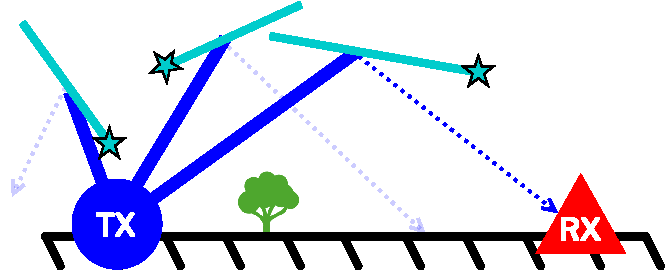
\includegraphics[height=1.8cm]{img/increase_power.pdf}%
            \end{center}%
            When many meteors reflect too little power to \textcolor{red}{\textbf{RX}} to be detected
        \end{column}
        \vrule{}
        \begin{column}[t]{0.35\textwidth}
            \begin{center}
                \alert{Increase network density}
                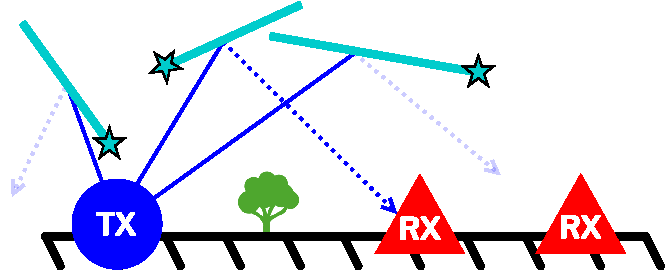
\includegraphics[height=1.8cm]{img/increase_density.pdf}%
            \end{center}%
            When many meteors reflect power away from most \textcolor{red}{\textbf{RX}}s
        \end{column}
        \vrule{}
        \begin{column}[t]{0.35\textwidth}
            \begin{center}
                \alert{Expand network coverage}
                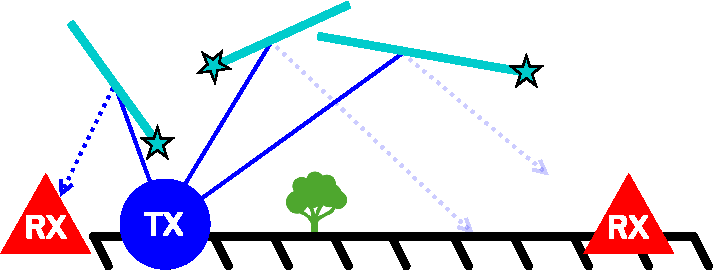
\includegraphics[height=1.8cm]{img/increase_coverage.pdf}%
            \end{center}%
            When most viable meteors are already detected
        \end{column}
    \end{columns}
\end{frame}

\begin{frame}[label=better_sci]
    \frametitle{Understanding Performance for Better Science}
    \begin{columns}
        \begin{column}{0.7\textwidth}
            \begin{exampleblock}{Example: ML Wind Field Estimation}
                With a 7x increase in observations, HYPER wind field estimation can resolve much finer physical features.
            \end{exampleblock}
            \begin{itemize}
                \item[\(\blacktriangleright\)] \hl{Are there that many more meteors available to see?}
                \item[\(\blacktriangleright\)] If so, how do we invest in networks to see them?  
            \end{itemize}

            % All estimation techniques benefit from more observations
            % \begin{itemize}
            %     \item[\(\blacktriangleright\)] The ability to design a high-performing network could bring new science
            %     \item[\(\blacktriangleright\)] Important to understand observational limits 
            % \end{itemize}
        \end{column}
        \begin{column}{0.3\textwidth}
            \centering 
            \begin{tikzpicture}
                \node[inner sep =0] (img) {
                    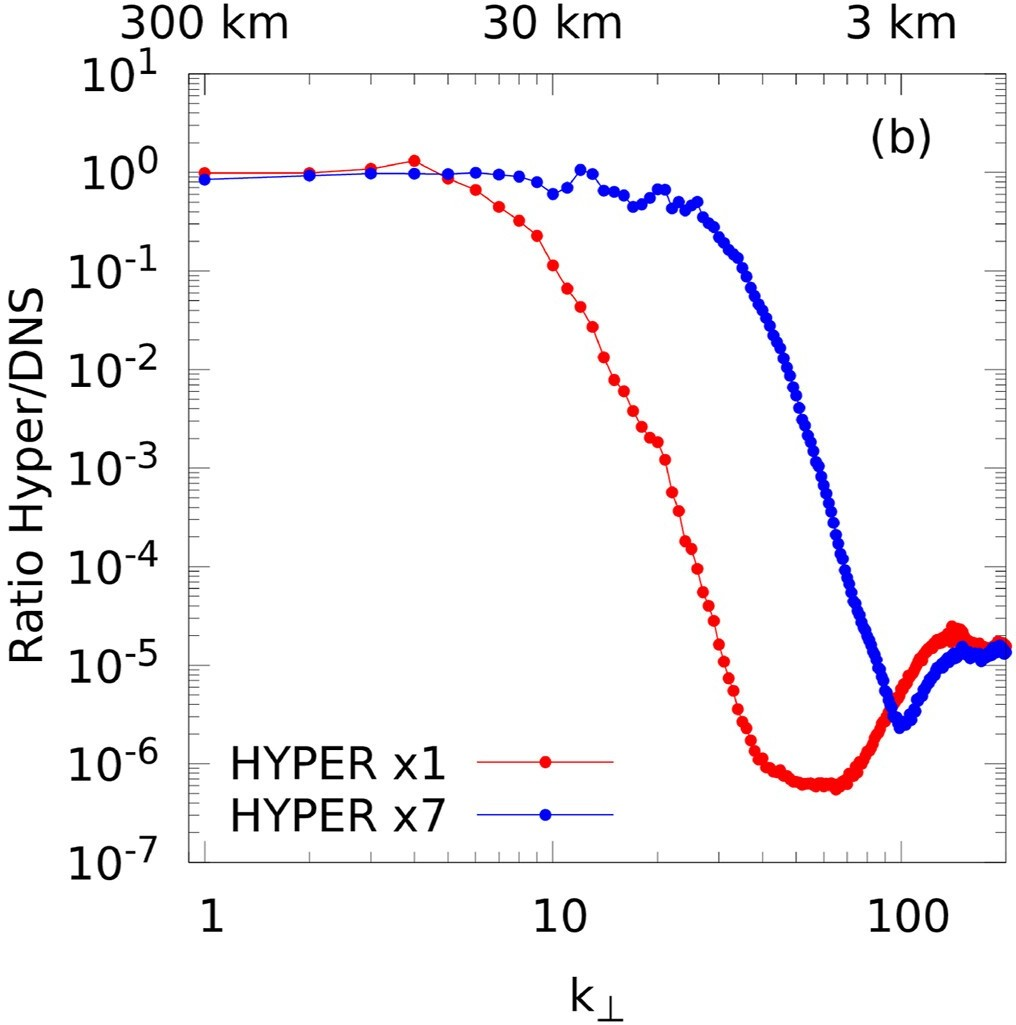
\includegraphics[width=\linewidth]{img/Hyper_urco.jpg}
                };
                \node[anchor = south east] at ([yshift = 0.7cm]img.south east) { 
                    {\fontsize{5}{5.4}\selectfont \textcolor{black}{Credit: \citeauthor{urco_AugmentedFourdimensionalMesosphere_2024}, \citeyear{urco_AugmentedFourdimensionalMesosphere_2024}  \cite{urco_AugmentedFourdimensionalMesosphere_2024}}}
                };
            \end{tikzpicture}
        \end{column}
    \end{columns}
\end{frame}